


\section{问题一的模型建立与求解}
\label{sec:method1}

\subsection{求解TSP问题的常见算法}
TSP(Traveling Salesman Problem)可描述为:给定一系列城市和每对城市之间的距离,求解访问每一座城市一次并回到起始城市的最短回路。它是组合优化中的一个NP-hard问题,在运筹学和理论计算机科学中非常重要.
TSP问题在1930年首次被形式化, 并且是在最优化中研究最深入的问题之一, 许多优化方法都用它作为一个基准. 尽管问题在计算上很困难, 但已经有了大量的启发式和精确方法, 比如遗传算法\cite{geneticTSP},模拟退火算法\cite{SimulatedAnnealing}, 蚁群算法\cite{AntTSP}, 甚至可以完全求解城市数量上万的实例, 并且甚至能在误差1\%范围内估计上百万个城市的问题\cite{AdlemanTSP}.

纯形式的TSP都可以应用到各行各业, 如企划, 物流, 芯片制造中的电路规划. 稍作修改, 就是DNA测序等许多领域的一个子问题. 在这些应用中, "城市" 的概念用来表示客户, 焊接点或DNA片段, "距离" 的概念表示旅行时间或成本或DNA片段之间的相似性度量. 

在本文中, 我们通过Sec.\ref{sec:preliminary}阐述的SOM模型对TSP问题进行求解.


%\subsubsection{数据预处理} %
%观察坐标点发现所有坐标点位置在$p=(120,36)$附近, 为了后续算法的稳定性, 我们将坐标统一增加$(-120,-
%36)$作为偏置.

\subsection{SOM模型解决TSP问题}
本节探讨如何通过SOM解决TSP问题, 该方法通过SOM网络的保序性来求解最短路径, 其应用最早在1988年被Angeniol和Fort提出\cite{som-tsp}.前文已经介绍了SOM模型基本概念, 其中对输出层(竞争层)一般抽象为六边形或矩形网格排列, 在TSP问题中, 更习惯将其抽象为环装\cite{som-tsp}. 对旅行商问题而言, 二维城市坐标是网络的输入向量, 城市空间位置关系是 SOM 要学习的模式, 而网络的输出是一个环形的神经元结构.


\begin{figure}[h]
    \begin{center}
        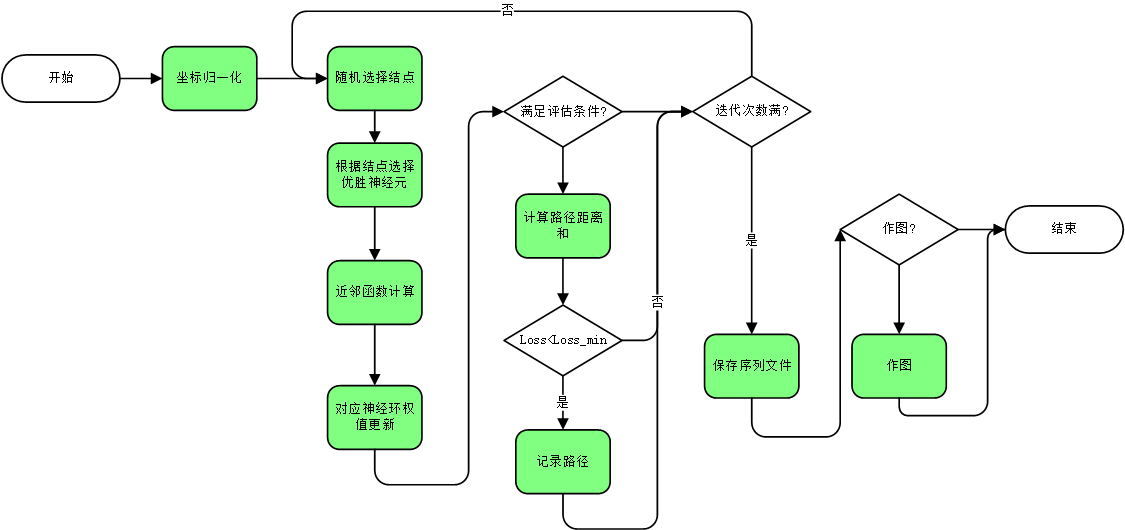
\includegraphics[width=0.95\linewidth]{fig/som-pipline}
    \end{center}
    \caption{\textbf{SOM方法流程图.} }
        \label{fig:som-pipline}
  \end{figure}


本文模型在随机选择, 优胜结点索引, 权值更新处与一般SOM模型一致, 在临近赋权时构建一维高斯函数, 对环装结点进行赋权.模型首先将节点坐标归一化, 去除偏置, 并在每次训练,获胜神经元及其近邻神经元的权值向量都会更新,经过多次反复的竞争与更新,神经网络最终学到输入数据的模式(结点的空间关系),并以神经元权值向量的形式保存下来, 体现在地图中,就是神经元的位置不断靠近城市的过程. 在解决TSP问题时, 神经元之间的竞争等价于寻找优胜神经元, 合作则等价于最优神经元更新时会带动周围其他神经元一起改变位置, 最终这会使得任意迭代步数的神经元环都能解算出一条对应的哈密顿回路, 求解的流程图如图\ref{fig:som-pipline}所示.






    
\subsection{som-TSP模型求解}

\begin{figure}[h]
    \begin{center}
        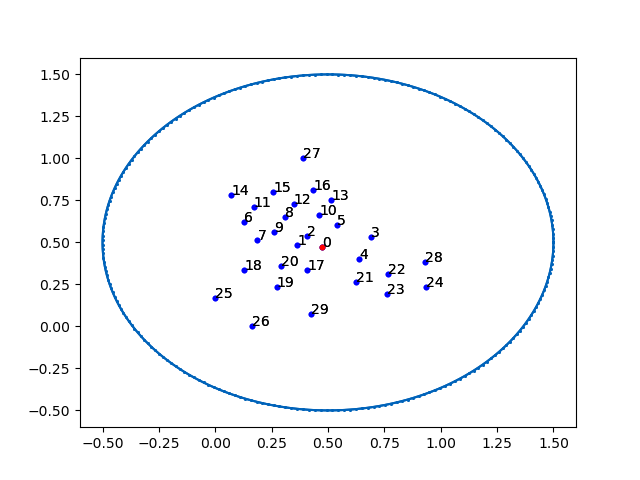
\includegraphics[width=0.55\linewidth]{fig/init}
    \end{center}
    \caption{\textbf{som-TSP模型神经环初始化.} 在求解过程中,点的坐标已经被归一化 }
        \label{fig:init}
  \end{figure}
  我们通过建立的som-TSP模型,对问题进行求解\footnote{som-TSP模型代码见支撑材料或\url{https://github.com/xdr940/som-TSP}}. 模型网络设为单层, 输出层共计210个神经元, 初始化神经环为圆形, 包裹所有点,如图\ref{fig:init}. 
模型共计迭代5000次, 每100次评估一次,评估指标为当前神经环解算出的回路总距离, 并将每次最好的结果保存. som-TSP模型求解时间在Intel I7 8700K上共计4.9s, 在第2500 次迭代中求出的最优路径, 如图\ref{fig:solution}, 长度为$L=0.1143807$, 换算后为$l = 11.43807km$. 路径为:

$p_{0}\rightarrow p_2\rightarrow p_1\rightarrow p_9\rightarrow p_7\rightarrow p_6\rightarrow p_{14}\rightarrow p_{11}\rightarrow p_{8}\rightarrow  p_{12}\rightarrow  p_{15}\rightarrow  p_{27}\rightarrow  p_{16}\rightarrow  p_{13}\rightarrow  p_{10}\rightarrow p_{5}\rightarrow p_{3}\rightarrow p_{4}\rightarrow p_{22}\rightarrow  p_{28}\rightarrow p_{24}\rightarrow p_{23}\rightarrow p_{21}\rightarrow p_{29}\rightarrow p_{26}\rightarrow p_{25}\rightarrow p_{18}\rightarrow p_{19}\rightarrow p_{20}\rightarrow p_{17}$


\begin{figure}[h]
    \begin{center}
        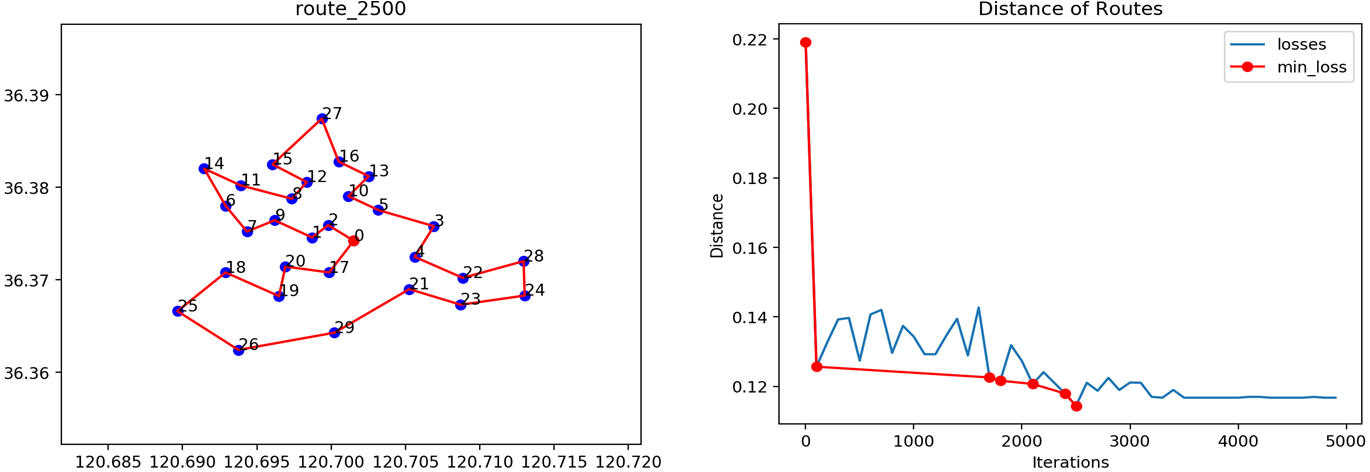
\includegraphics[width=1.0\linewidth]{fig/solution}
    \end{center}
    \caption{\textbf{最优解路径与迭代过程中路径变化.} }
        \label{fig:solution}
  \end{figure}






\begin{figure}[h]
    \begin{center}
        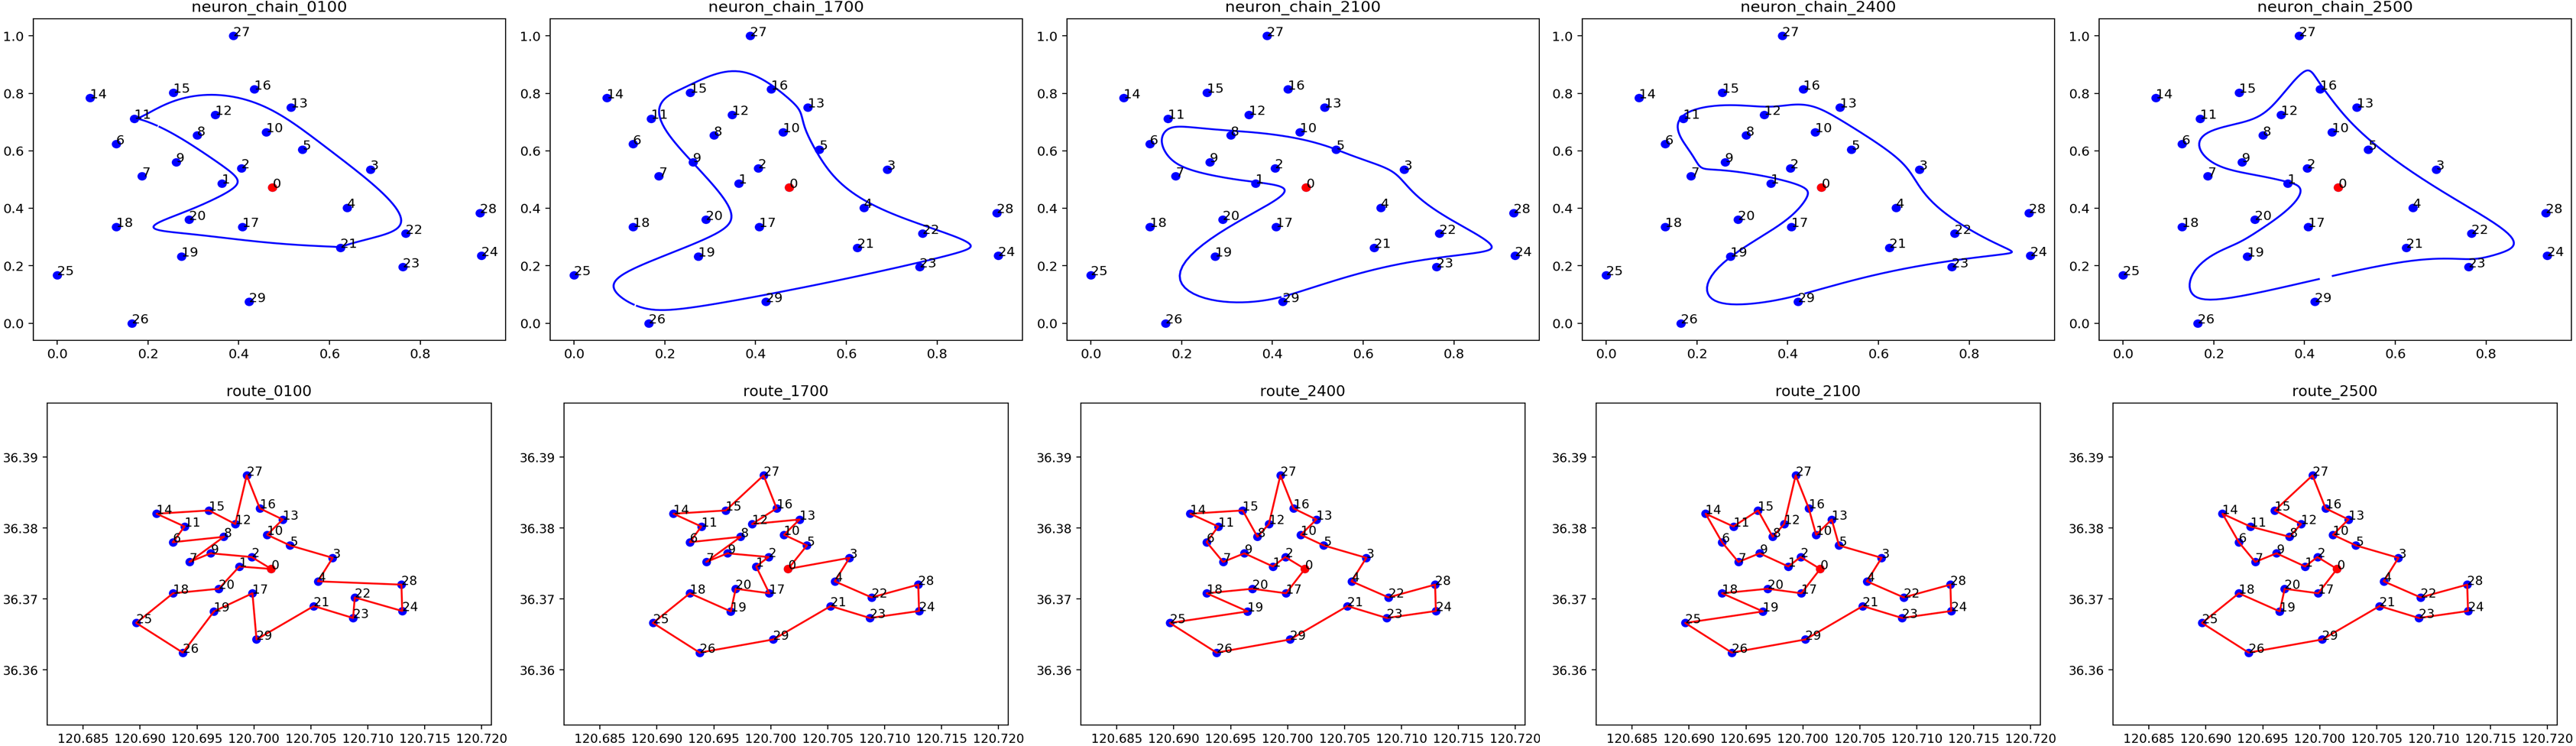
\includegraphics[width=1.0\linewidth]{fig/iteration}
    \end{center}
    \caption{\textbf{som-TSP模型求解过程.}第一行为神经元环可视化,第二行为神经元环对应的解} 
        \label{fig:iteration}
  \end{figure}